\chapter{Die Programmiersprache WHILE} \label{chap:while}

Die in dieser Arbeit entwickelte Programmiersprache ist Turing-Vollständig und prozedural. Es existiert ein einziger Datentyp: positive ganze Zahlen. Es ist nicht möglich eigene Datentypen oder Klassen zu definieren, es können jedoch beliebig viele Variablen und Funktionen definiert und genutzt werden. Die Programmiersprache orientiert sich stark an den beiden Programmiersprachen \enquote{loop} und \enquote{while}, welche im neunten Kapitel im Buch \citetitle{GottfriedVossen2016} von \citeauthor{GottfriedVossen2016} beschrieben werden. \cite{GottfriedVossen2016} 

\section{Kommentare}
Wie aus vielen anderen Programmiersprachen bekannt, kann der Programmcode mithilfe von zwei führenden Schrägstrichen  kommentiert werden.

\section{Variablen}
Variablendeklarationen werden mit dem Schlüsselwort \textbf{var} gekennzeichnet. Darauf folgt der Name der Variable. Anders als in anderen Programmiersprachen ist es hier notwendig der Variable bei der Deklaration auch einen Wert zuzuweisen. Eine Zuweisung erfolgt mit einem Doppelpunkt gefolgt von einem Gleichheitszeichen (:=). Einer Variable können Konstanten, Variablen oder Funktionsaufrufe zugewiesen werden. Nachdem eine Variable erzeugt wurde kann ihr ein neuer Wert zugewiesen werden oder sie in Funktionsaufrufen genutzt werden.

\begin{lstlisting}[language=c, caption=Variablennutzung in While, label={lst:while-var-defdec}]
var r0 := 0; // Erzeugt eine Variable mit dem Namen 'r0' und dem Wert 0
var r1 := r0; // Erzeugt eine Variable mit dem Namen 'r1' und dem Wert von r0
r0 := 5; // r0 bekommt einen neuen Wert
\end{lstlisting}

\section{Pred und Succ}
\textbf{pred} und \textbf{succ} sind zwei Funktionen, welche die Sprache zur Verfügung stellt und den Wert von einer Variable direkt manipulieren können. Nach dem jeweiligen Schlüsselwort folgt der Name einer Variable innerhalb von zwei runden Klammern. \textbf{pred} steht für \enquote{predecessor} und wird genutzt um den Wert einer Variable um eine Stelle zu verringern. Analog dazu wird \textbf{succ} (\enquote{successor}) genutzt um den Wert einer Variable zu erhöhen. Der Wert einer Variable kann beliebig oft erhöht werden, der kleinste Wert einer Variable ist jedoch immer null.

\begin{lstlisting}[language=c, caption=pred und succ in While, label={lst:while-var-defdec}]
	var r0 := 1; // Erzeugt eine Variable mit dem Namen 'r0' und dem Wert 1
	pred(r0); // Der Wert ist nun 0
	succ(r0); // Der Wert ist nun 1
\end{lstlisting}

\section{Loop und While}
\textbf{loop} und \textbf{while} sidn zwei unterschiedliche Schleifenarten, welche in der Programmiersprache while genutzt werden können. Der Schleifenkörper befindet sich in beiden Fällen einem \textbf{begin:} und \textbf{end}. Innerhalb eines Schleifenkörpers können beliebig viele Anweisungen oder auch andere Schleifen stehen. Variablen, welche innerhalb eines Schleifenkörpers definiert werden, existieren nur innerhalb vom Schleifenkörper.

Die \textbf{while} Schleife verhält sich, wie man es aus anderen Sprachen gewohnt ist: der Körper der Schleife wird wiederholt, solange der Wert der Variable im Schleifenkopf ungleich null ist. Mithilfe einer \textbf{while}-Schleife ist es möglich Endlosschleifen zu erzeugen.

\begin{lstlisting}[language=c, caption=while-Schleife in While, label={lst:while-var-defdec}]
	var r0 := 3; // Erzeugt eine Variable mit dem Namen 'r0' und dem Wert 3
	while(r0) begin: // Die Schleife laeuft solange r0 != 0
		pred(r0); // Veraender den Wert von r0
	end
\end{lstlisting}

Die \textbf{loop} Schleife hingegen verhält sich ähnlich zu einer for-Schleife aus anderen Programmiersprache. Die Variable im Schleifenkopf wird automatisch verringert bis der Wert gleich null ist. Aus diesem Grund kann davon ausgegangen werden, dass die Schleife terminiert. Um das sicher zu stellen, ist es bei einer \textbf{loop}-Schleife nicht möglich die Variable, welche im Schleifenkopf steht, schreibend zu verwenden. 

\begin{lstlisting}[language=c, caption=loop-Schleife in While, label={lst:while-var-defdec}]
	var r0 := 3; // Erzeugt eine Variable mit dem Namen 'r0' und dem Wert 3
	loop(r0) begin: // r0 wird bei jedem Durchlauf automatisch verringert
		var r1 := r0; // Der Wert von r0 darf gelesen werden.
		pred(r0); // Es ist innerhalb der Schleife verboten den Wert zu aendern!
	end
\end{lstlisting}

\section{Read und Write}
\textbf{read} und \textbf{write} sind zwei Funktionen, welche genutzt werden können um zur Laufzeit mit dem Benutzer des Programms zu interagieren. Mithilfe von \textbf{read} wird der Nutzer aufgefordert der angegeben Variable über eine Tastatureingabe einen Wert zuzuweisen. 

\begin{lstlisting}[language=c, caption=read in While, label={lst:while-var-defdec}]
	var r0 := read(); // Bitten den Nutzer einen Wert fuer r0 anzugeben
\end{lstlisting}

Mithilfe von \textbf{write} kann der Wert von einer Variable, welche in runden Klammern angegeben wird, auf die Konsole ausgegeben werden, um dem Nutzer beispielsweise ein Rechenergebnis anzuzeigen. Es ist möglich mehrere Variablen gleichzeitig auszugeben, dazu können mehrere Klammern innerhalb der runden Klammern angegeben werden, die Variablen jeweils mit einem Komma voneinander getrennt. 

\begin{lstlisting}[language=c, caption=write in While, label={lst:while-var-defdec}]
	var r0 := 3; // Erzeugt eine Variable mit dem Namen 'r0' und dem Wert 3
	var r1 := 2; // Erzeugt eine Variable mit dem Namen 'r0' und dem Wert 3
	write(r0); // Gibt den Wert von r0 auf die Konsole aus
	write(r0, r1); // Gibt den Wert von r0 und r1 auf die Kosole aus
\end{lstlisting}

\section{Funktionen}
Um den Programmcode besser zu organisieren existieren Funktionen. Eine Funktionsdefinition beginnt mit \textbf{def} und kann beliebig viele Parameter haben und muss immer einen Wert zurück geben. Parameter stehen in runden Klammern und werden mit Kommata voneinander getrennt, sie werden als Kopie vom original Wert übergeben. Der Funktionskörper steht, ähnlich wie bei Schleifen, zwischen \textbf{begin:} und \textbf{end}. Ein \textbf{return} um einen Wert zurück zu geben darf immer nur am Schluss einer Funktion stehen. 

\begin{lstlisting}[language=c, caption=Funktionen in While, label={lst:while-var-defdec}]
	def addTwo(s0) begin: // Definiere eine Funktion
		succ(s0);
		succ(s0);
		return s0; // Gebe einen Wert zurueck
	end
	var r0 := 3; // Erzeugt eine Variable mit dem Namen 'r0' und dem Wert 3
	var r1 := addTwo(r0); // Erzeugt eine Variable mit dem Namen 'r1' und dem Wert von addTwo(r0)
\end{lstlisting}
\section{Grammatik}
Die Konzepte, welche in \cref{sec:while-konzepte} vorgestellt wurden, wurden in einer Form beschrieben, die für Menschen gut verständlich ist. Ein Computerprogramm, wie beispielsweise ein Compiler, benötigt eine andere Form der Erklärung, wie der Aufbau eines Programmcodes auszusehen hat. Diese Erklärung erfolgt mithilfe von unterschiedlichen  Grammatikregeln, welche in der sogenannten \ac{ebnf} aufgeschrieben werden. Ein Beispiel für zwei Grammatikregel ist in \cref{lst:while-grammar-pred} zu sehen.

\begin{lstlisting}[language=c, caption=Zwei einfache Grammatikregel, label={lst:while-grammar-pred}]
	ID:    [a-zA-Z][a-zA-Z0-9]*;
	pred: 'pred' '(' ID ')' ';';
\end{lstlisting}

In der ersten Zeile ist zu sehen, wie eine \textbf{ID} aufgebaut sein muss, sie muss mit einem kleinen Buchstaben beginnen und darauf dürfen beliebig viele Zahlen und Buchstaben folgen. Eine \textbf{ID} entspricht einem Funktions- oder Variablennamen.  In der nächsten Zeile ist zu sehen, wie eine \textbf{pred}-Anweisung auszusehen hat (\cref{subsec:while-konzepte-pred}).

Grammatikregeln können sehr gut in Form von sogennanten \enquote{Railroad-,} oder {Syntaxdiagrammen} dargestellt werden, wodurch sie einfach zu verstehen sind. Beispielsweise ist in \cref{pic:WhileRegelWhile} das Syntaxdiagramm für eine while-Schleife zu sehen. Darin ist beispielsweise erkennbar, dass eine leere Schleife in der entwickelten Programmiersprache zulässig wäre, genau so wie eine Schleife mit beliebig vielen Statements.

\begin{figure}[h!]
	\centering
	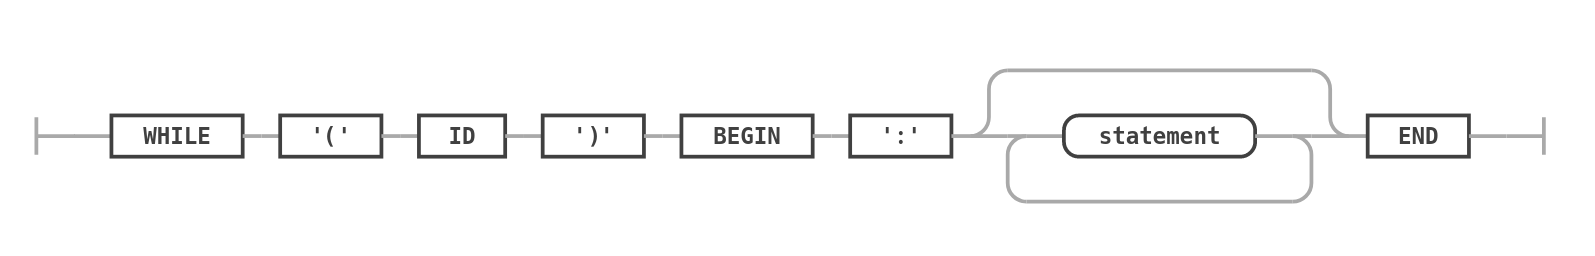
\includegraphics[width=14cm]{content/pictures/while.png}
	\caption{Die Grammatikregel für eine while-Schleife}
	\label{pic:WhileRegelWhile}
\end{figure}

Wie ein Statement definiert wird, ist in \cref{pic:WhileRegelStatement} zu erkennen. Als Statement werden viele unterschiedliche Konzepte bezeichnet: ein \textbf{succ} und \textbf{pred} sind statements oder auch \textbf{while} und \textbf{loop}. Aus den beiden Diagrammen lässt sich schließen, dass die Sprache auch Schleifen innerhalb von while-Schleifen erlaubt, was auch der Fall ist. 

\begin{figure}[h!]
	%\includegraphics[width=1\textwidth]{content/pictures/LoRaWAN-OSI.JPG}
	\centering
	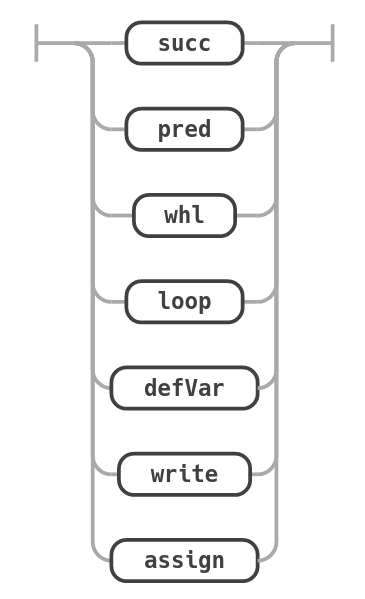
\includegraphics[width=4cm]{content/pictures/statement.png}
	\caption{Die Grammatikregel für ein Statement}
	%	\source{\cite[S. 5]{SemtechCorporation.2020}}
	\label{pic:WhileRegelStatement}
\end{figure}

Wenn ein Programm einer Menge von Grammatikregeln entspricht, bedeutet das nicht zwingend, dass der Programmcode fehlerfrei ist. Es existieren Fehleingaben, welche nur schwer durch Grammatikregeln erkannt werden können. Beispielsweise erlaubt die oben gezeigte Grammatik eine Wertzuweisung ohne vorauszusetzen, dass die entsprechende Variable zuvor definiert wurde. Um solche Fehler zu erkennen wird eine sogenannte semantische Analyse durchgeführt. Dieses Thema wird in \cref{chap:semantic} behandelt.


